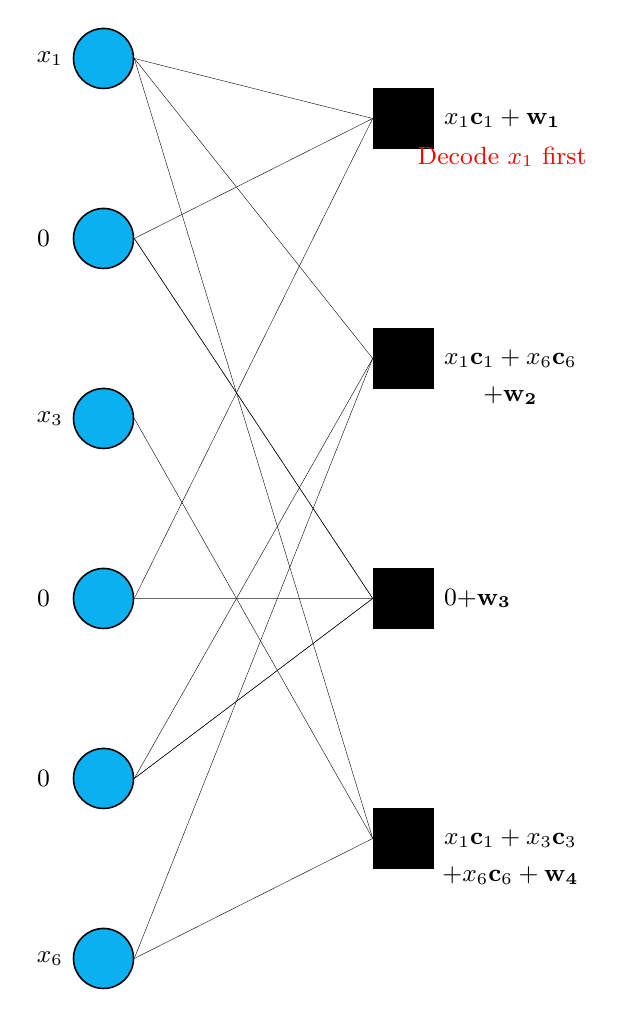
\begin{tikzpicture}
\def\horzgap{1.5in}; %Horizontal gap between nodes/levels
\def \gapVN{0.9in}; %vertical gap between nodes
\def \gapCN{1.2in}; %Horizontal gap between nodes


\def\nodewidth{0.3in};
\def\nodewidthA{0.3in};
\def \edgewidth{0.12in};
\def\ext{1.2in};

\def\fsize{\small};

\tikzstyle{check} = [rectangle, draw,line width=0.2mm,  inner sep=0mm, fill=black, minimum height=\nodewidthA, minimum width=\nodewidthA]
\tikzstyle{bit} = [circle, draw, line width=0.2mm, inner sep=0mm, fill=ProcessBlue, minimum size=\nodewidthA]
\tikzstyle{bituncover} = [circle, draw=none, line width=0.2mm, inner sep=0mm, fill=gray, minimum size=\nodewidthA]

\tikzstyle{edgesock} = [circle, inner sep=0mm, minimum size=\edgewidth,draw, fill=white]     

                          
\foreach \vn in {1,...,6}{
 \node[bit] (vn\vn) at (0,-\vn*\gapVN) {};
}

\foreach \vn in {2,4,5}{
\path (vn\vn) ++(-\nodewidth,0) node()[inner sep=0mm] {\fsize{0}};
}

\node[anchor=east, left] at (vn1.west){\fsize{$x_{1}$}};
\node[anchor=east, left] at (vn3.west){\fsize{$x_{3}$}};
\node[anchor=east, left] at (vn6.west){\fsize{$x_{6}$}};

\foreach \cn in {1,...,4}{
\node[check] (cn\cn) at (\horzgap,-\cn*\gapCN) {};
}

\draw[line width=0.05mm] (vn6.east)--(cn4.west);
\draw[line width=0.05mm] (vn3.east)--(cn4.west);
\draw[line width=0.05mm] (vn1.east)--(cn4.west);

\draw[line width=0.05mm] (vn2.east)--(cn3.west);
\draw[line width=0.05mm] (vn4.east)--(cn3.west);
\draw[line width=0.05mm] (vn5.east)--(cn3.west);

\draw[line width=0.05mm] (vn2.east)--(cn3.west);
\draw[line width=0.05mm] (vn4.east)--(cn3.west);
\draw[line width=0.05mm] (vn5.east)--(cn3.west);

\draw[line width=0.05mm] (vn6.east)--(cn2.west);
\draw[line width=0.05mm] (vn5.east)--(cn2.west);
%\draw[line width=0.05mm] (vn3.east)--(cn2.west);
\draw[line width=0.05mm] (vn1.east)--(cn2.west);

\draw[line width=0.05mm] (vn1.east)--(cn1.west);
\draw[line width=0.05mm] (vn2.east)--(cn1.west);
\draw[line width=0.05mm] (vn4.east)--(cn1.west);

\def\moveX {1.8*\nodewidth};
\def\moveXA {2*\nodewidth};

\node(cn1text)[anchor=west,right] at (cn1.east) {\fsize{$x_1\mathbf{c}_1+\mathbf{w_{1}}$}};
\node[anchor=north,below] at (cn1text.south) {\fsize{\textcolor{red}{Decode $x_1$ first}}};
\node[anchor=west,right](cn2text) at (cn2.east){\fsize{$x_1\mathbf{c}_1+x_6\mathbf{c}_6$}};
\node[below] at (cn2text.south) {\fsize{$+\mathbf{w_{2}}$}};
\node[anchor=west,right] at (cn3.east) {\fsize{0+$\mathbf{w_{3}}$}};
\node[anchor=west,right](cn4text) at (cn4.east) {\fsize{$x_1\mathbf{c}_1+x_3\mathbf{c}_3$}};
\node[anchor=north, below] at (cn4text.south) {\fsize{$+x_6\mathbf{c}_6+\mathbf{w_{4}}$}};
%-----------------------*(&^#@$^&*(^%$^&*(&^--------------------------------------------------------------------

\end{tikzpicture}